\documentclass[letterpaper]{article}

\usepackage{hyperref}
\usepackage{tikz}

\title{Amazon Delivery Truck Simulation}
\author{Hanna Butt \thanks{HFB352} \and Ashton Cole \thanks{AVC687, \href{mailto:ashtonc24@utexas.edu}{ashtonc24@utexas.edu}} \and Kelechi Emeruwa \thanks{KEE688}}
\date{\today}

\begin{document}
    \maketitle

    \begin{abstract}
        Summary of whole paper. Note that this is not an introduction or context, but a summary.
    \end{abstract}

    \section{Introduction}
    \label{section:Introduction}
    Introduce the context and the problem here. Also talk about project context (we're in COE 322 fall 2022, this is a final group project, bla bla bla).

    Here's a paragraph that lays out a roadmap for the report. In Section \ref{section:Methodology} we discuss the algorithm used to solve the simple Traveling Salesman Problem, and expansions upon it to construct our final program. In Section \ref{section:Results}, we display the outcomes of several test scenarios and discuss the results. Finally, in Section \ref{section:Conclusion}, we offer our final thoughts and reflect on ethical considerations.

    \section{Methodology}
    \label{section:Methodology}
    Notes: Talk about how we're solving the problem (C++, TACC super computer) and how the program works (e.g. reads in text file, spits out text file). Then go into the development process/timeline (we started simple with address/list classes, tested functionality, and then expand it a bit)

    In Section \ref{subsection:Software_and_Hardware}, we discuss the means by which we conducted our simulations. In Section \ref{subsection:Object-Oriented_Structure}, we outline the structure of the classes used to represent and solve the probelm. In Section \ref{subsection:Traveling_Salesman_Problem}, we describe the algorithms we used to solve the simple Traveling Salesman Problem. In Section \ref{subsection:Multiple_Traveling_Salesman_Problem}, we describe the expansion of the problem to account for optimizing multiple delivery routes. [more intermediate developments could go here] Finally, in Section \ref{subsection:Developing_the_Final_Product}, we describe how we combined our algorithms into a final product for a hypothetical user.

    \subsection{Software and Hardware}
    \label{subsection:Software_and_Hardware}
    Go into detail about how we're using C++, we're using TACC's isp machine, what that is, \&c.

    \subsection{Object-Oriented Structure}
    \label{subsection:Object-Oriented_Structure}

    \subsection{Traveling Salesman Problem}
    \label{subsection:Traveling_Salesman_Problem}

    Talk about greedy and opt2 algorithms.

    \begin{figure}[h]
        \caption{An unsorted Route is optimized through both the greedy algorithm (blue) and the opt2 algorithm (green). This demonstrates how the opt2 algorithm alone is not necessarily sufficient to find the shortest Route.}
        \label{figure:sortdemo}
        \begin{minipage}{0.3\linewidth}
            % Old
            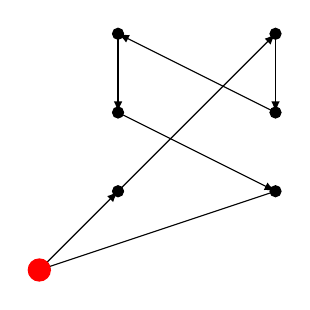
\begin{tikzpicture}
                \draw [black, -latex] (0, 0) -- (1, 1);
                \filldraw [black] (0, 0) circle (2pt);
                \draw [black, -latex] (1, 1) --(3, 3);
                \filldraw [black] (1, 1) circle (2pt);
                \draw [black, -latex] (3, 3) --(3, 2);
                \filldraw [black] (3, 3) circle (2pt);
                \draw [black, -latex] (3, 2) --(1, 3);
                \filldraw [black] (3, 2) circle (2pt);
                \draw [black, -latex] (1, 3) --(1, 2);
                \filldraw [black] (1, 3) circle (2pt);
                \draw [black, -latex] (1, 2) --(3, 1);
                \filldraw [black] (1, 2) circle (2pt);
                \draw [black, -latex] (3, 1) --(0, 0);
                \filldraw (3, 1) [black] circle (2pt);
                \filldraw [red] (0, 0) circle (4pt);
            \end{tikzpicture}
        \end{minipage}
        \begin{minipage}{0.3\linewidth}
            % Greedy
            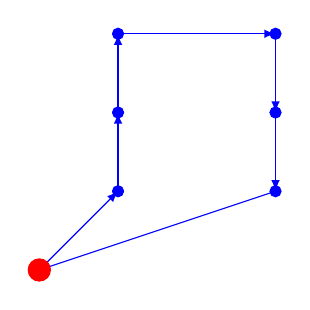
\begin{tikzpicture}
                \draw [blue, -latex] (0, 0) -- (1, 1);
                \filldraw [blue] (0, 0) circle (2pt);
                \draw [blue, -latex] (1, 1) --(1, 2);
                \filldraw [blue] (1, 1) circle (2pt);
                \draw [blue, -latex] (1, 2) --(1, 3);
                \filldraw [blue] (1, 2) circle (2pt);
                \draw [blue, -latex] (1, 3) --(3, 3);
                \filldraw [blue] (1, 3) circle (2pt);
                \draw [blue, -latex] (3, 3) --(3, 2);
                \filldraw [blue] (3, 3) circle (2pt);
                \draw [blue, -latex] (3, 2) --(3, 1);
                \filldraw [blue] (3, 2) circle (2pt);
                \draw [blue, -latex] (3, 1) --(0, 0);
                \filldraw (3, 1) [blue] circle (2pt);
                \filldraw [red] (0, 0) circle (4pt);
            \end{tikzpicture}
        \end{minipage}
        \begin{minipage}{0.3\linewidth}
            % opt2
            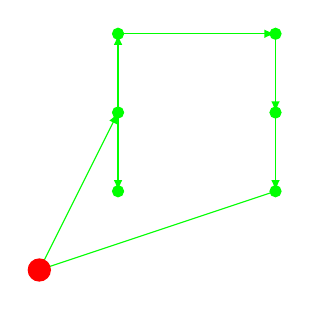
\begin{tikzpicture}
                \draw [green, -latex] (0, 0) -- (1, 2);
                \filldraw [green] (0, 0) circle (2pt);
                \draw [green, -latex] (1, 2) --(1, 1);
                \filldraw [green] (1, 2) circle (2pt);
                \draw [green, -latex] (1, 1) --(1, 3);
                \filldraw [green] (1, 1) circle (2pt);
                \draw [green, -latex] (1, 3) --(3, 3);
                \filldraw [green] (1, 3) circle (2pt);
                \draw [green, -latex] (3, 3) --(3, 2);
                \filldraw [green] (3, 3) circle (2pt);
                \draw [green, -latex] (3, 2) --(3, 1);
                \filldraw [green] (3, 2) circle (2pt);
                \draw [green, -latex] (3, 1) --(0, 0);
                \filldraw (3, 1) [green] circle (2pt);
                \filldraw [red] (0, 0) circle (4pt);
            \end{tikzpicture}
        \end{minipage}
    \end{figure}

    \subsection{Multiple Traveling Salesman Problem}
    \label{subsection:Multiple_Traveling_Salesman_Problem}
    Talk about how swap algorithm works. Figure \ref{figure:swapdemo} provides a simple example of how this algorithm improves the total distance. (Now prove it with data! What are the distances before and after?)

    \begin{figure}[h]
        \caption{Two Routes exchange Addresses to optimize their distances.}
        \label{figure:swapdemo}
        \begin{minipage}{0.45\linewidth}
            % Unswapped
            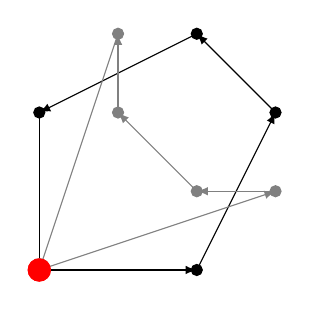
\begin{tikzpicture}
                % Route 1
                \draw [black, -latex] (0, 0) -- (2, 0);
                \filldraw [black] (0, 0) circle (2pt);
                \draw [black, -latex] (2, 0) --(3, 2);
                \filldraw [black] (2, 0) circle (2pt);
                \draw [black, -latex] (3, 2) --(2, 3);
                \filldraw [black] (3, 2) circle (2pt);
                \draw [black, -latex] (2, 3) --(0, 2);
                \filldraw [black] (2, 3) circle (2pt);
                \draw [black, -latex] (0, 2) --(0, 0);
                \filldraw (0, 2) [black] circle (2pt);
                \filldraw [red] (0, 0) circle (4pt);
                % Route 2
                \draw [gray, -latex] (0, 0) -- (3, 1);
                \filldraw [gray] (0, 0) circle (2pt);
                \draw [gray, -latex] (3, 1) --(2, 1);
                \filldraw [gray] (3, 1) circle (2pt);
                \draw [gray, -latex] (2, 1) --(1, 2);
                \filldraw [gray] (2, 1) circle (2pt);
                \draw [gray, -latex] (1, 2) --(1, 3);
                \filldraw [gray] (1, 2) circle (2pt);
                \draw [gray, -latex] (1, 3) --(0, 0);
                \filldraw (1, 3) [gray] circle (2pt);
                \filldraw [red] (0, 0) circle (4pt);
            \end{tikzpicture}
        \end{minipage}
        \begin{minipage}{0.45\linewidth}
            % Swapped
            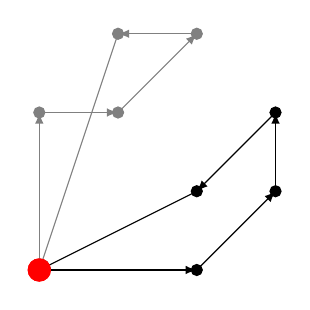
\begin{tikzpicture}
                % Route 1
                \draw [black, -latex] (0, 0) -- (2, 0);
                \filldraw [black] (0, 0) circle (2pt);
                \draw [black, -latex] (2, 0) --(3, 1);
                \filldraw [black] (2, 0) circle (2pt);
                \draw [black, -latex] (3, 1) --(3, 2);
                \filldraw [black] (3, 1) circle (2pt);
                \draw [black, -latex] (3, 2) --(2, 1);
                \filldraw [black] (3, 2) circle (2pt);
                \draw [black, -latex] (2, 1) --(0, 0);
                \filldraw (2, 1) [black] circle (2pt);
                \filldraw [red] (0, 0) circle (4pt);
                % Route 2
                \draw [gray, -latex] (0, 0) -- (0, 2);
                \filldraw [gray] (0, 0) circle (2pt);
                \draw [gray, -latex] (0, 2) --(1, 2);
                \filldraw [gray] (0, 2) circle (2pt);
                \draw [gray, -latex] (1, 2) --(2, 3);
                \filldraw [gray] (1, 2) circle (2pt);
                \draw [gray, -latex] (2, 3) --(1, 3);
                \filldraw [gray] (2, 3) circle (2pt);
                \draw [gray, -latex] (1, 3) --(0, 0);
                \filldraw (1, 3) [gray] circle (2pt);
                \filldraw [red] (0, 0) circle (4pt);
            \end{tikzpicture}
        \end{minipage}
    \end{figure}

    %%%%%
    %%%%%
    %%%%%
    %%%%% MORE DEVELOPMENT STEPS COULD GO HERE
    %%%%%
    %%%%%
    %%%%%

    \subsection{Developing the Final Product}
    \label{subsection:Developing_the_Final_Product}
    How is our final thing going to work? Basically we want it to work for businesses.

    \section{Results}
    \label{section:Results}
    Pretty pictures and tables go here. Describe each situation being displayed and talk about what they mean, e.g. is it the optimal solution? Good enough? Is there a tradeoff between time to execute and quality of results?

    Hmm, maybe insert a table comparing number of nodes/trucks to program execution time. What rate does it increase at $(O(n), O(n^2), \&c.)$

    \subsection{Scenario 1}

    \subsection{Scenario 2}

    \subsection{Performance Data}
    go over execution time and stuff

    \section{Conclusion}
    \label{section:Conclusion}
    Talk about what we learned, how this all applies to industry, ideas to scale the problem up, ethics, \&c.
\end{document}